\chapter{ARQUITETURA DO MODELO}

O modelo proposto é uma arquitetura de \textbf{Rede Neural Artificial Profunda} com dados heterogêneos de texto e imagem. Seu formato é a combinação de outras arquiteturas já conhecidas e amplamente utilizadas para resolver separadamente problemas de \textbf{Processamento de Linguagem Natural} e \textbf{Visão Computacional}. 

\begin{figure}[htb]
	\caption{\label{arquitetura_macro_do_modelo} Arquitetura Macro do Modelo}
	\begin{center}
	    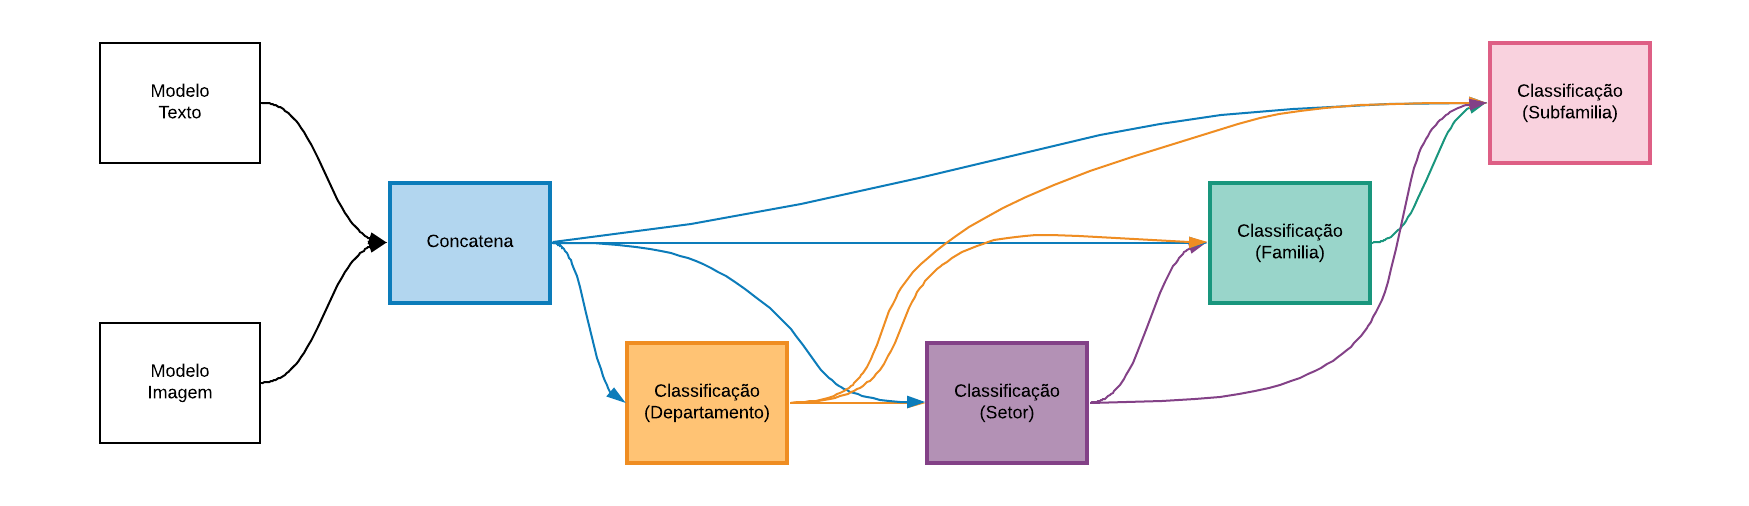
\includegraphics[width=\textwidth]{artigo/recursos/imagens/arquitetura_macro_do_modelo.png}
	\end{center}
	\legend{Fonte: Elaborado pelo Autor}
\end{figure}

Para viabilizar a utilização de dados heterogêneos simultaneamente no modelo. São utilizados dois blocos distintos na rede neural para a extração dos atributos de cada tipo de dado. Para então combinar esses atributos em um conjunto maior que serão injetados nas redes densas de classificação. Vale notar que a saída do nível acima faz parte da entrada do próximo nível.

\section{MODELO DE TEXTO}

O modelo responsável por extrair os atributos dos textos dos produtos, utiliza várias técnicas para atingir este objetivo e pode ser visto na \autoref{modelo_macro_texto}.

\begin{figure}[htb]
	\caption{\label{modelo_macro_texto} Arquitetura Macro do Modelo de texto}
	\begin{center}
	    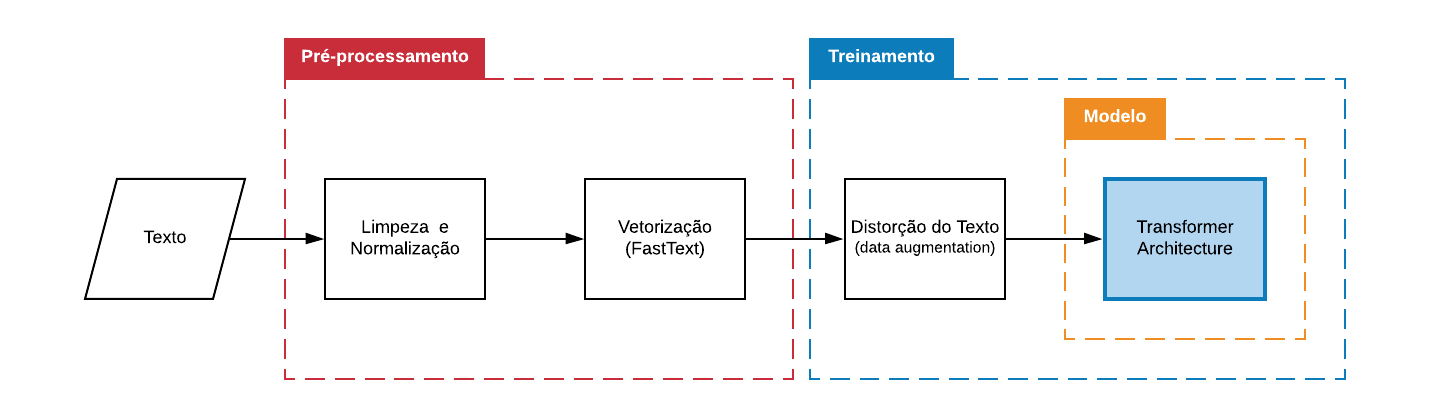
\includegraphics[width=\textwidth]{artigo/recursos/imagens/modelo_macro_texto.png}
	\end{center}
	\legend{Fonte: Elaborado pelo Autor}
\end{figure}

Sendo o FastText para a conversão do texto em uma representação vetorial.
para extrair atributos (features) das palavras, distorção do texto, Posicionamento das palavras na sequência e Self-Attention.

\subsection{PRÉ PROCESSAMENTO DO TEXTO}

Todo o texto utilizado passa por uma função de normalização a fim de remover a maior quantidade de inconsistências e simplificar seu formato. A função de normalização pode ser encontrada no \autoref{chap:funcao_normalizacao_texto}.

\subsection{VETORIZAÇÃO DO TEXTO}

A representação do texto de forma vetorial para que possa ser utilizada nos modelos de aprendizado de máquina. Essas representações precisam ser simples e que contenham em si as informações sobre o significado das palavras.

Para o nosso caso, obtivemos melhores resultados usando o \textbf{FasText} proposto no artigo \cite{fasttext}. Esse método de representação vetorial é interessante, pois diferente do \textbf{CBOW} e \textbf{SKIP-GRAM} introduzidos no artigo \cite{mikolov}, o FastText é capaz de representar palavras que não foram vistas durante o treinamento o que é uma grande vantagem com a variável de palavras e modelos que normalmente seguem um padrão para a sua formação, como no exemplo à seguir, onde apenas muda um carácter no modelo do smartphone.

\begin{itemize}
\item Smartphone Samsung Galaxy \textbf{S10} ...
\item Smartphone Samsung Galaxy \textbf{S10e} ...
\item Smartphone Samsung Galaxy \textbf{S10+} ...
\end{itemize}

\subsubsection{REPRESENTAÇÃO DAS PALAVRAS}

As palavras são representadas pela soma da representação vetorial de seus \textit{n-grams} mais um termo especial que é a própria palavra se ela esteja presente no dicionário. Caso a palavra não esteja presente no dicionário, então ela só será representada somente pela soma de seus \textit{n-grams}.

Note que na \autoref{fasttext_representacao_das_palavras_ngram_com_especial} a palavra “água” aparecer como um termo especial, enquanto na \autoref{fasttext_representacao_das_palavras_ngram_sem_especial} o termo especial não aparece, dando a ideia de que não esta presente no dicionário, portanto a representação das palavras são feitas somente pelos seus \textit{n-grams}.

\begin{figure}[htb]
	\caption{\label{fasttext_representacao_das_palavras_ngram_com_especial} Representação das palavras conhecidas}
	\begin{center}
	    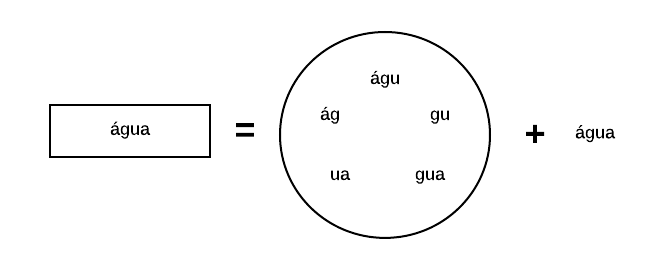
\includegraphics[scale=1.0]{artigo/recursos/imagens/fasttext_representacao_das_palavras_ngram_com_especial.png}
	\end{center}
	\legend{Fonte: Elaborado pelo Autor}
\end{figure}

\begin{figure}[htb]
	\caption{\label{fasttext_representacao_das_palavras_ngram_sem_especial} Representação das palavras desconhecidas}
	\begin{center}
	    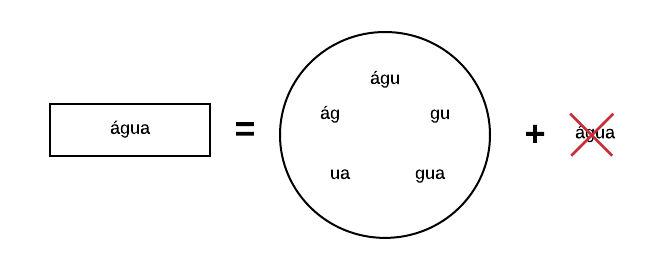
\includegraphics[scale=1.0]{artigo/recursos/imagens/fasttext_representacao_das_palavras_ngram_sem_especial.png}
	\end{center}
	\legend{Fonte: Elaborado pelo Autor}
\end{figure}

Vale notar que o FastText já possui diversos modelos pré-treinados em várias línguas e podem ser encontradas no seu site \href{https://fasttext.cc/docs/en/english-vectors.html}{FastText Models}.

No entanto, para maximizar a performance do modelo, foi necessário fazer um treinamento especializado com os dados do e-commerce. Para mais detalhes, veja o APÊNDICE F.

\subsubsection{MODELO FASTTEXT}

O modelo do FastText é uma variação do \textbf{skip-gram} introduzido no \cite{mikolov}, onde dado uma sequencia de palavras o objetivo é maximizar a probabilidade do contexto dado as palavras em volta. Um exemplo dessa ideia pode ser visto na \autoref{examplo_skip_gram}.

\begin{figure}[htb]
	\caption{\label{examplo_skip_gram} Exemplo do contexto dado as palavras em volta}
	\begin{center}
	    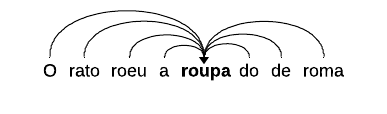
\includegraphics[scale=1.0]{artigo/recursos/imagens/examplo_skip_gram.png}
	\end{center}
	\legend{Fonte: Elaborado pelo Autor}
\end{figure}

Dado um vocabulário de tamanho $W$, cada palavra é identificada pelo seu índice $w \in {1, .., W}$ tendo o objetivo de criar uma representação vetorial para cada palavra neste dicionário.

Dado uma sequência de palavras $w_1, ..., w_T$ o objetivo do modelo skip-gram é maximizar a probabilidade do contexto dado as palavras ao seu redor.

\begin{center}\large
    $\sum_{t=1}^{T} \sum_{c \in C_t} log(p(w_c | w_t))$
\end{center}

função de pontuação

\begin{center}\large
    $s(w, c) = \sum_{g \in G_w} z_{g}^{T} v_c$
\end{center}

logistic loss function

\begin{center}\large
    $l(x) = log(1 + e^{-x})$
\end{center}

\begin{center}\large
    $\sum_{t=1}^{T} = \left [ \sum_{c \in C_t} l(s(w_t, w_c))) + \sum_{n \in N_{t,c}} l(-s(w_t, n)) \right ]$
\end{center}

\subsection{DISTORÇÃO DO TEXTO}

Para tornar o treinamento mais genérico possível e com maior variabilidade dos dados, é utilizado dois tipos de distorção no texto (data augmentation), sendo a primeira a de remover palavras e a segunda de inverter a ordem de palavras de forma randômica e uniforme. As funções que implementam essa funcionalidade estão disponíveis no APÊNDICE - B.

FIGURA 3: Exemplo da utilização das funções de distorção de texto

FONTE: Elaborado pelo Autor

\subsection{TRANSFORMER ARCHITECTURE}

A arquitetura Transformer Architecture (“Attention is all you need” [2]) foi escolhida para ser utilizada como mecanismo para a extração de features do texto dada a sua capacidade de paralelização e acurácia.

FIGURA X: Arquitetura do modelo Transformer

FONTE: “Attention is All You Need” [2] de 2017

A arquitetura é constituída de dois principais blocos. O Codificador (Encoder) e o Decodificador (Decoder) para fazer a tradução de textos. Para o nosso contexto, que é a classificação de produtos, é utilizado somente o bloco Codificador que pode ser visto na FIGURA X.

FIGURA X: 

FONTE: Produzida pela autor

Vale notar, que na implementação atual, é utilizado somente um bloco do Codificador onde foi possível obter excelentes resultados. Ficando para trabalhos futuros averiguar a necessidade de adicionar mais blocos, criando uma pilha de codificadores.

\subsubsection{EMBEDDING INPUT}

O “embedding Input” é uma (Xijd) sequência vetorial de tamanho pré-definido que é a representação do texto em formato de matriz, onde essa matriz é gerada pelo FastText e então distorcida.

Xi,jd

One i é o tamanho do lote (batch), j é o tamanho da sequência (quantidade de palavras) e d é a quantidade de dimensões do vetor das palavras (tamanho da saído do vetor do FastText). 

O tamanho de j varia conforme o conjunto de dados de treinamento, e busca informar qual o tamanho adequado da quantidade máxima de palavras que será utilizado para formar as sequências removendo as discrepâncias (“outliers”) e reduzindo assim a complexidade do modelo. Essa quantidade é definida à partir de:

%A = {c0 ... cn}| A está ordenada
%k = ⌈p(n+1) / 100⌉

Onde A é uma sequência ordenada da quantidade de palavras por exemplo do conjunto de dados de treinamento,  p-ésimo é a parte  do conjunto de dados que estamos buscando (foi utilizado o valor de p igual à 99,7) e n é o tamanho da amostra, ambos os valores são calculados à partir do conjunto de dados de treinamento. O resultado k é o posição de A que representa a quantidade de palavras que será utilizada.

\subsubsection{CODIFICAÇÃO POSICIONAL}

Nesta etapa, o objetivo é adicionar a informação de posição nas sequências. Isso se faz necessário, pois o modelo não possui consciência do que é posição, diferente de uma Rede Neural Recorrente. A função para a codificação das sentenças se dá por:

Onde d é o tamanho do vetor dos palavras da sequências e i é um vetor de tamanho d que representa as posições de cada atributo do vetor de palavras.

Enquanto pos é uma matriz do tamanho do l,m onde l é o tamanho do lote e m é a quantidade de palavras na sequência.

Um exemplo do código que faz essa implementação pode ser visto no APÊNDICE X - CODIFICAÇÃO POSICIONAL.

\subsubsection{MULTI-HEAD SELF-ATTENTION}
O que é Attention

A definição de Mecanismo de Atenção (“Attention Mechanism”) consiste em “Each annotation hi contains information about whole input sequence with a strong focus on the partes surrounding the i-th word of the input sequence” de acordo com [2], em tradução direta “Cada anotação hi contém informação sobre toda a sentença, com ênfase nas partes que rodeiam a palavra i-th da sequência de entrada”.
É possível observar que a ideia consiste em em criar um contexto para cada palavra na sequência onde determinadas palavras têm mais relevância do que outras.
Onde o contexto ci é criado pelo somatório do produto dos pesos aij com as palavras. Onde os pesos são calculados para todas as palavras usando a função softmax.

O que é self attention

o que Multi-Head self-attention


\subsubsection{CONEXÃO RESIDUAL E NORMALIZAÇÃO}
asdsad

\subsubsection{CAMADA DENSA}
asdasd


\section{IMAGEM}

Para complementar e ampliar ainda mais a quantidade de informações para fazer a classificação, introduzimos nesta versão do modelo a utilização de imagens. A ideia aqui consiste em capturar características do produto que não estão disponíveis em seus títulos.
Vale notar que nesta versão, só utilizamos a imagem principal dos produtos.

FIGURA 4: Visualização modelo de imagem

FONTE: Elaborado pelo autor


\subsection{DISTORÇÃO DAS IMAGENS}

Assim como foi feito nos textos, também é feito a distorção (data augmentation) nas imagens para tornar o treinamento melhor e mais genérico, pois toda vez que uma imagem passa pela rede, é como se fosse uma nova imagem. Para atingir esse objetivo é empregado diversas modificações nas imagens como pode ser visto no exemplo da FIGURA X.

FIGURA X: Exemplo de distorções em Imagens

FONTE: Elaborado pelo autor

O código fonte das distorções, pode ser visto no APÊNDICE E.

\subsection{ARQUITETURA RESNET V2}

Como arquitetura para a extração de features é utilizado a ResNet V2 

\section{CONJUNTO DE DADOS}
Como não há uma possibilidade no momento de criar um conjunto de dados anotados manualmente, utilizamos os produtos já classificados previamente.     Com isso, o conjunto de dados é separado em três partes:

conjunto de dados de treinamento (inclui técnica de oversampling e undersampling)
conjunto de dados de validação (utilizado para acompanhar a performance do modelo durante o treinamento é usado na cláusula de parada)

conjunto de dados de teste (utilizado para criar o relatório final)

\subsection{SELEÇÃO DO CONJUNTO DE DADOS}

Para tentar criar um conjunto de dados razoável, precisamos tomar como premissa de que os dados que possuímos estão corretos e são aplicados as seguintes técnicas:

Para tentar reduzir o ruído no conjunto de dados, é utilizado um modelo de auxiliar capaz de identificar possíveis produtos mal categorizados;

Quanto os produtos de uma subfamília possuem quantidade menor ou igual à 3, essas subfamílias são removidas pois não possuem dados o suficiente para treinar, validar e testar;

Uma vez o conjunto de dados selecionado, é feito a separação dos dados de treinamento, validação e teste. Onde 90 dos dados são para treinamento, 5 para validação e 5 para teste. Os dados de treinamento passam ainda por oversampling e undersampling.
Para as subfamílias com muitos produtos, são feitas o undersampling definindo um máximo de a Média mais duas vezes o Desvio padrão (mean + 2*std);
Para as subfamílias com produtos menores que 30, é feito o oversampling (replicação de exemplos) até ficarem com 30 amostras.

\section{TREINAMENTO}

O treinamento do modelo ocorre utilizando 8 GPUs Nvidia V100 durante X dias e para somente baseado na cláusula de parada que pode ser visto na seção 2.4.3 CLÁUSULA DE PARADA. 

\subsection{OTIMIZADOR}

Para o otimizador é utilizado mini-batch (128) com SGD com Momentum e Nesterov a fim de aumentar a velocidade do treinamento com o learning rate inicial de 0,01 e sendo reduzido após a décima época num fator exponencial.

\subsection{FUNÇÃO DE ERRO (LOSS FUNCTION)}

Como os dados são extremamentes desbalanceados e em certas classes tem tão poucos e outras grandes quantidades de exemplos e a variabilidade e sutileza, buscamos na literatura uma função de erro que fosse capaz de incluir esse desbalanceamento durante o treinamento.
O Focal Loss é uma variação do Cross Entropy especializado em dados desbalanceados desenvolvido para detectar objetos sob fundos em imagens. Foi desenvolvido no Facebook AI Research (LIN et al., 2017). A publicação esta disponível em: https://arxiv.org/abs/1708.02002 e o código fonte de exemplo está disponível no APÊNDICE C.
ADICIONAR FUNÇÃO MATEMÁTICA

\subsection{CLÁUSULA DE PARADA}

É definido como cláusula de parada, quando o modelo para de conseguir reduzir o loss do conjunto de dados de validação com uma paciência de 10 épocas.
